\documentclass{tufte-book}

%\hypersetup{colorlinks}% uncomment this line if you prefer colored hyperlinks (e.g., for onscreen viewing)

%%
% If they're installed, use Bergamo and Chantilly from www.fontsite.com.
% They're clones of Bembo and Gill Sans, respectively.
%\IfFileExists{bergamo.sty}{\usepackage[osf]{bergamo}}{}% Bembo
%\IfFileExists{chantill.sty}{\usepackage{chantill}}{}% Gill Sans

%\usepackage{microtype}

%%
% For nicely typeset tabular material
\usepackage{booktabs}

%%
% For graphics / images
\usepackage{graphicx}
\setkeys{Gin}{width=\linewidth,totalheight=\textheight,keepaspectratio}
\graphicspath{{graphics/}}

% The fancyvrb package lets us customize the formatting of verbatim
% environments.  We use a slightly smaller font.
\usepackage{fancyvrb}
\fvset{fontsize=\normalsize}

%%
% Prints argument within hanging parentheses (i.e., parentheses that take
% up no horizontal space).  Useful in tabular environments.
\newcommand{\hangp}[1]{\makebox[0pt][r]{(}#1\makebox[0pt][l]{)}}

%%
% Prints an asterisk that takes up no horizontal space.
% Useful in tabular environments.
\newcommand{\hangstar}{\makebox[0pt][l]{*}}

%%
% Prints a trailing space in a smart way.
\usepackage{xspace}

%%
% Some shortcuts for Tufte's book titles.  The lowercase commands will
% produce the initials of the book title in italics.  The all-caps commands
% will print out the full title of the book in italics.
\newcommand{\vdqi}{\textit{VDQI}\xspace}
\newcommand{\ei}{\textit{EI}\xspace}
\newcommand{\ve}{\textit{VE}\xspace}
\newcommand{\be}{\textit{BE}\xspace}
\newcommand{\VDQI}{\textit{The Visual Display of Quantitative Information}\xspace}
\newcommand{\EI}{\textit{Envisioning Information}\xspace}
\newcommand{\VE}{\textit{Visual Explanations}\xspace}
\newcommand{\BE}{\textit{Beautiful Evidence}\xspace}

\newcommand{\TL}{Tufte-\LaTeX\xspace}

% Prints the month name (e.g., January) and the year (e.g., 2008)
\newcommand{\monthyear}{%
  \ifcase\month\or January\or February\or March\or April\or May\or June\or
  July\or August\or September\or October\or November\or
  December\fi\space\number\year
}


% Prints an epigraph and speaker in sans serif, all-caps type.
\newcommand{\openepigraph}[2]{%
  %\sffamily\fontsize{14}{16}\selectfont
  \begin{fullwidth}
  \sffamily\large
  \begin{doublespace}
  \noindent\allcaps{#1}\\% epigraph
  \noindent\allcaps{#2}% author
  \end{doublespace}
  \end{fullwidth}
}

% Inserts a blank page
\newcommand{\blankpage}{\newpage\hbox{}\thispagestyle{empty}\newpage}

\usepackage{units}

% Typesets the font size, leading, and measure in the form of 10/12x26 pc.
\newcommand{\measure}[3]{#1/#2$\times$\unit[#3]{pc}}

% Macros for typesetting the documentation
\newcommand{\hlred}[1]{\textcolor{Maroon}{#1}}% prints in red
\newcommand{\hangleft}[1]{\makebox[0pt][r]{#1}}
\newcommand{\hairsp}{\hspace{1pt}}% hair space
\newcommand{\hquad}{\hskip0.5em\relax}% half quad space
\newcommand{\TODO}{\textcolor{red}{\bf TODO!}\xspace}
\newcommand{\ie}{\textit{i.\hairsp{}e.}\xspace}
\newcommand{\eg}{\textit{e.\hairsp{}g.}\xspace}
\newcommand{\na}{\quad--}% used in tables for N/A cells
\providecommand{\XeLaTeX}{X\lower.5ex\hbox{\kern-0.15em\reflectbox{E}}\kern-0.1em\LaTeX}
\newcommand{\tXeLaTeX}{\XeLaTeX\index{XeLaTeX@\protect\XeLaTeX}}
% \index{\texttt{\textbackslash xyz}@\hangleft{\texttt{\textbackslash}}\texttt{xyz}}
\newcommand{\tuftebs}{\symbol{'134}}% a backslash in tt type in OT1/T1
\newcommand{\doccmdnoindex}[2][]{\texttt{\tuftebs#2}}% command name -- adds backslash automatically (and doesn't add cmd to the index)
\newcommand{\doccmddef}[2][]{%
  \hlred{\texttt{\tuftebs#2}}\label{cmd:#2}%
  \ifthenelse{\isempty{#1}}%
    {% add the command to the index
      \index{#2 command@\protect\hangleft{\texttt{\tuftebs}}\texttt{#2}}% command name
    }%
    {% add the command and package to the index
      \index{#2 command@\protect\hangleft{\texttt{\tuftebs}}\texttt{#2} (\texttt{#1} package)}% command name
      \index{#1 package@\texttt{#1} package}\index{packages!#1@\texttt{#1}}% package name
    }%
}% command name -- adds backslash automatically
\newcommand{\doccmd}[2][]{%
  \texttt{\tuftebs#2}%
  \ifthenelse{\isempty{#1}}%
    {% add the command to the index
      \index{#2 command@\protect\hangleft{\texttt{\tuftebs}}\texttt{#2}}% command name
    }%
    {% add the command and package to the index
      \index{#2 command@\protect\hangleft{\texttt{\tuftebs}}\texttt{#2} (\texttt{#1} package)}% command name
      \index{#1 package@\texttt{#1} package}\index{packages!#1@\texttt{#1}}% package name
    }%
}% command name -- adds backslash automatically
\newcommand{\docopt}[1]{\ensuremath{\langle}\textrm{\textit{#1}}\ensuremath{\rangle}}% optional command argument
\newcommand{\docarg}[1]{\textrm{\textit{#1}}}% (required) command argument
\newenvironment{docspec}{\begin{quotation}\ttfamily\parskip0pt\parindent0pt\ignorespaces}{\end{quotation}}% command specification environment
\newcommand{\docenv}[1]{\texttt{#1}\index{#1 environment@\texttt{#1} environment}\index{environments!#1@\texttt{#1}}}% environment name
\newcommand{\docenvdef}[1]{\hlred{\texttt{#1}}\label{env:#1}\index{#1 environment@\texttt{#1} environment}\index{environments!#1@\texttt{#1}}}% environment name
\newcommand{\docpkg}[1]{\texttt{#1}\index{#1 package@\texttt{#1} package}\index{packages!#1@\texttt{#1}}}% package name
\newcommand{\doccls}[1]{\texttt{#1}}% document class name
\newcommand{\docclsopt}[1]{\texttt{#1}\index{#1 class option@\texttt{#1} class option}\index{class options!#1@\texttt{#1}}}% document class option name
\newcommand{\docclsoptdef}[1]{\hlred{\texttt{#1}}\label{clsopt:#1}\index{#1 class option@\texttt{#1} class option}\index{class options!#1@\texttt{#1}}}% document class option name defined
\newcommand{\docmsg}[2]{\bigskip\begin{fullwidth}\noindent\ttfamily#1\end{fullwidth}\medskip\par\noindent#2}
\newcommand{\docfilehook}[2]{\texttt{#1}\index{file hooks!#2}\index{#1@\texttt{#1}}}
\newcommand{\doccounter}[1]{\texttt{#1}\index{#1 counter@\texttt{#1} counter}}

% Generates the index
\usepackage{makeidx}
\makeindex


\usepackage{indentfirst}

\usepackage[utf8]{inputenc}
\usepackage[T1]{fontenc}

%%%%%%%%%%%%%%%%%%%%%%%%%%%%%%%% Customization %%%%%%%%%%%%%%%%%%%%%%%%%%%%%%%%

\setcounter{tocdepth}{1}
\setcounter{secnumdepth}{0}

\renewcommand\contentsname{\normalfont \huge Table des matières}

\titlecontents{chapter}%
    [0em]% distance from left margin
    {\vspace{1\baselineskip}\begin{fullwidth}Chapitre }% above (global formatting of entry)
    {\contentslabel{0em} \hspace{1em} \huge $\vert$ \Large}% before w/ label (label = ``Chapter 1'')
    {\hspace{1em}}% before w/o label
    {\hfill\qquad\thecontentspage}% filler and page (leaders and page num)
    [\end{fullwidth}]% after
\titlecontents{section}% FIXME
    [0em] % distance from left margin
    {\vspace{0\baselineskip}\begin{fullwidth} \rmfamily\itshape} % above (global formatting of entry)
    {\hspace*{6em}\contentslabel{2em}} % before w/label (label = ``2.6'')
    {\hspace*{7em}} % before w/o label
    {\normalfont\hfill\qquad\thecontentspage} % filler + page (leaders and page num)
    [\end{fullwidth}] % after


\begin{document}

% Front matter
\frontmatter

%%%%%%%%%%%%%%%%%%%%%%%%%%%%%%%%%%%% Titre %%%%%%%%%%%%%%%%%%%%%%%%%%%%%%%%%%%%

\newpage
\author{Quentin Lobbé}
\title{\nohyphenation{Archives et Fragments Web}}
\cleardoublepage
{  
  \begin{fullwidth}%
  \thispagestyle{empty} 
  \setlength{\parskip}{\baselineskip}
  \begingroup
  \vspace*{10em}
  \par\noindent\Large{Quentin Lobbé}
  \vspace*{-1em}
  \par\noindent\Huge\textbf{Archives et Fragments Web}
  \par\noindent\nohyphenation\Large{Désagréger les archives Web pour mener une exploration temporelle de traces numériques des migrations}
  \endgroup
  \vfill  
  \par\noindent\nohyphenation Université Paris-Saclay, École doctorale des sciences et technologies de l'information et de la communication.  Thèse pour l'obtention du doctorat de Télécom ParisTech et de l'Université Paris-Saclay.    
  \end{fullwidth}%
}

\blankpage

%%%%%%%%%%%%%%%%%%%%%%%%%%%%%%%%%%%% Info Thèse %%%%%%%%%%%%%%%%%%%%%%%%%%%%%%%%%%%%
  
\newpage
\begin{fullwidth}
~\vfill
\thispagestyle{empty}
\setlength{\parskip}{\baselineskip}

\par\noindent Thèse présentée par \textbf{\thanklessauthor}\\
LTCI, Télécom ParisTech, Université Paris Saclay \& Inria. Paris, France.\\
quentin.lobbe@telecom-paristech.fr

\par\noindent Sous la direction de :\\
\textbf{Pierre Senellart}, professeur à l'École Normale Supérieure\\
\textbf{Dana Diminescu}, professeure à Télécom ParisTech

\par\noindent Soutenue publiquement à Paris le 9 novembre 2018, devant un jury composé de :\\
\textbf{Bruno Bachimont} (Rapporteur), enseignant-chercheur à l'Université Technologique de Compiègne\\
\textbf{Marc Spaniol} (Rapporteur), professeur à l'Université de Caen Basse-Normandie\\
\textbf{Anat Ben-David}, professeure à l'Open University of Israel\\
\textbf{Dominique Cardon}, professeur associé à Sciences Po Paris\\
\textbf{Bruno Defude}, directeur adjoint de la recherche et des formations doctorales à Télécom SudParis

\par\textit{last modified \monthyear}
\end{fullwidth}
  
\thispagestyle{empty}%
\clearpage%

%%%%%%%%%%%%%%%%%%%%%%%%%%%%%%%% Remerciements %%%%%%%%%%%%%%%%%%%%%%%%%%%%%%%%

\newpage

~\vfill
\noindent
\justify
\par\noindent Il me demanda de chercher la première page.\\
\noindent Je posais ma main gauche sur la couverture et ouvris le volume de mon pouce serré contre l'index. Je m'efforçais en vain : il restait toujours des feuilles entre la couverture et mon pouce. Elles semblaient sourdre du livre.\\
- Maintenant cherchez la dernière.\\
\noindent Mes tentatives échouèrent de même; à peine pus-je balbutier d'une voix qui n'était plus ma voix :\\
- Cela n'est pas possible.\\
\noindent Toujours à voix basse le vendeur me dit : \\
- Cela n'est pas possible et pourtant cela \textit{est}. Le nombre de pages de ce livre est exactement infini. Aucune n'est la première, aucune n'est la dernière.
\\~\\
\noindent\textit{Jorge Luis Borges - Le livre de sable} 
\vfill
\indent
\newpage
\begingroup
\vspace*{8em}
\huge $\vert$ \huge Remerciements
\vspace*{4em}
\par\normalsize Ici je remercie plein de gens

\par Beaucoup de gens

\par Mais vraiment
\endgroup
\vfill

%%%%%%%%%%%%%%%%%%%%%%%%%%%%%%%%%%%% Tables %%%%%%%%%%%%%%%%%%%%%%%%%%%%%%%%%%%%

\tableofcontents

\listoffigures

\listoftables

\mainmatter

%%%%%%%%%%%%%%%%%%%%%%%%%%%%%%%%%% Chapitre 1 %%%%%%%%%%%%%%%%%%%%%%%%%%%%%%%%%%

\chapter{Introduction}

\section{Introduction générale}

Ici l'intro de la thèse.

\section{Mise en garde}

\subsection{Penser le passé depuis le présent}

Ici on fait un rapide détour par l'historiographie et les difficultés à parler du passé depuis le présent.

\subsection{Conservation différentielle et nature des archives Web}

Ici on parle de la raréfaction de la matière Web à mesure que l'on remonte le temps et également à mesure que le web fournit du contenu.

%%%%%%%%%%%%%%%%%%%%%%%%%%%%%%%%%% Chapitre 2 %%%%%%%%%%%%%%%%%%%%%%%%%%%%%%%%%%

\chapter{Du Web aux Représentations en Ligne des Diasporas}

\section{Retour aux origines du Web}

\section{Le migrant connecté}

\section{Le Web, espace de communication et d'organisation}

\section{L'Atlas e-Diasporas}

%%%%%%%%%%%%%%%%%%%%%%%%%%%%%%%%%% Chapitre 3 %%%%%%%%%%%%%%%%%%%%%%%%%%%%%%%%%%

\chapter{20 ans d'archivage du Web}

\section{Les pionniers}

Internet Archive et le pre-Unesco

\section{Préserver notre héritage numérique}

L'unesco et faire des archives un commun
Un tour du monde des initiatives 
La constitution juridique des corpus en france 
Et l'état de l'archivage aujourd'hui (fin de Internet mémory et les rogues archivistes)

\section{Constituer des corpus d'archives}

\subsection{Méthodologie d'acquisition}

Où l'on fait le tour de l'état de l'art en matière de création d'archives Web, de crawl, etc ...

\subsection{Un format unique ?}

Où l'on parle du WARC (et de ces prédécesseurs) vs le DAFF

\section{Les archives Web de l'Atlas e-Diasporas}

Présentation rapide de l'ensemble des corpus et focus sur les Marocains (expliquation ...)

%%%%%%%%%%%%%%%%%%%%%%%%%%%%%%%%%% Chapitre 4 %%%%%%%%%%%%%%%%%%%%%%%%%%%%%%%%%%

\chapter{Traces Discrétisées et Temporalité Figée}

\section{Détruire pour mieux archiver}

De Derrida aux traces discrétisées, de la sélection effectuée par le crawler et l'archiviste, les archives sont des traces discrètes du Web, comme Funes on ne peut tout garder 

\section{Un temps sans extension}

Ici on part de Saint Augustin et de sa définition d'un présent sans extension qui a influencer le rapport des occidentaux au temps. Ce rapport au temps se retrouve lorsque l'on étudie en détail les modèles d'exploration des archives web qui s'appuient sur la date de capture d'un contenu. S'en suit plusieurs remarques qu'il faut conserver en tete avant de se plonger dans toute exploration

\subsection{Crawl blindness}

\subsection{Cohérence}

\subsection{Duplicata}

\section{Construire un moteur d'exploration d'archive}

\subsection{Extraction et enrichissement}

\subsection{Définition du schéma d'indexation}

\subsection{Détection d'événements}

\section{Les archives sont des traces indirectes du Web}

Les archives sont les traces directes du crawler et non du web (Cf mises en gardes précédentes) + exemple sur yabiladi.com donc il faut descendre au niveau de la page et y extraire d'autres temporalités, d'autres forme d'exploration qui ne dépendent pas non plus de la linéarité proposé par les moteurs d'exploration classique.
La désagragation se fait dans le modèle de données mais également dans la façon de conduire sont exploration. 

%%%%%%%%%%%%%%%%%%%%%%%%%%%%%%%%%% Chapitre 5 %%%%%%%%%%%%%%%%%%%%%%%%%%%%%%%%%%

\chapter{Fragmenter les Archives Web}

\par\noindent Les effets de \textit{crawl legacy} sont indissociables des archives Web telles que nous les connaissons. Liés organiquement à la structure même des divers formats d'archivage, ils en sont les artéfacts directs et demeurent des obstacles majeurs pour qui souhaite mener à bien une exploration du Web archivé. S'il est tout à fait possible, depuis la WayBack Machine par exemple, de différencier \textit{à la main} la date d'archivage d'une page Web visitée de la date supposée de sa création ou de la date de publication réelle de tel ou tel contenu, cette tâche deviendra rapidement fastidieuse voire titanesque à mesure que grandira notre périmètre d'exploration. En associant les contenus archivés à la temporalité seule du crawler (voir \textbf{Figure X}), les archives Web se détachent de réalité historique des sites et des pages Web dont elles sont censées être le reflet fidèle. Ainsi, un site Web pourra être sur-représenté (ou inversement sous-représenté : voir \textbf{Figure X}) au sein d'un corpus d'archives au cours d'une période potentiellement plus liée à la programmation du crawler qu'à l'activité effective du site et des ses pages.   

L'exploration fine et complète de notre corpus d'archives sous-tend à toute compréhension de l'évolution de l'e-Diasporas marocaine telle que nous la formulions en Introduction. Tout l'enjeu de ce chapitre sera de déterminer un moyen d'affranchir les archives Web du lien qui les unissent aux crawlers. Il s'agira ici de retrouver, dans le code HTML des corpus archivés, les indices de la création d'une page ou de la publication d'un contenu et d'articuler notre analyse autour de ces nouvelles données : descendre au delà du niveau des Web. 

L'essentiel de ce chapitre sera donc consacré à ce déplacement, à ce changement d'échelle analytique (ou de strate au sens de N. Brügger \citep{brugger_website_2009}) et à ces conséquences. Au geste du crawler, nous substituerons le geste de l'auteur et du lecteur dont le passage sur les pages Web archivés aura laissé des traces qu'il nous faudra exploiter. Sur ce point, nous proposerons l'introduction d'une nouvelle unité d'exploration des archives Web : le \textit{fragment Web}. Nous présenterons, dans un premier temps, la genèse et les inspirations qui sous-tendent et motivent la définition du \textit{fragement Web}. Puis, nous reviendrons en miroir sur les modalités techniques et théoriques d'un moteur d'exploration d'archives Web telles que présentées dans le Chapitre 4, mais cette fois-ci, revisitées à l'aune du \textit{fragment Web}. Cette mise à niveau servira de base aux explorations présentées plus avant dans le Chapitre 6.

\section{5.1 Vers une nouvelle unité d'exploration}

\par\noindent Au delà de la simple volonté de s'affranchir des limitations du format actuel des archives Web, notre proposition de fragmenter les corpus d'archives est portée par l'idée selon laquelle toute archive est une matière destinée à être déconstruire, désagréger ou ré-arrangée en vue de la questionner et d'inventer l'histoire. Une archive ne parle pas seule \citep{ketelaar_de_2006}, elle n'est jamais fermée, jamais complète, mais se tient toujours prête à être réinterprétée par une nouvelle génération. Mais gardons néanmoins à l'esprit, comme le rappel J. Derrida\footnote{\textit{"je peux interroger, contredire, attaquer ou simplement déconstruire une logique du texte venu avant moi, devant moi, mais je ne peux ni ne dois le changer"} \cite{derrida_mal_1995}}, que le document d'origine (dans notre cas la page Web archivée) ne doit en aucun cas être altéré ou modifié. Et ce, pour justement permettre à d'autres, après nous, d'à nouveau s'y référer, le faire parler. 

Le \textit{fragment Web}, tel que nous le présenterons dans la suite de ce chapitre, ne sera donc pas une version modifiée d'une page Web archivée, mais bien une nouvelle entité issue de la page Web déconstruite et utilisable en parallèle des modèles d'exploration d'archives déjà existants.    

\subsection{Découper, déplacer, monter}

\par\noindent Nous évoquions déjà, dans le chapitre précédent, le personnage de Funes imaginé par J. L. Borges qui, dans la fable, est condamné à ne plus jamais rien oublier au détriment de ses propres capacités à penser. Funes se redécouvre ainsi sans cesse, n'arrivant pas à se créer des souvenirs, à se raconter de mémoire sa propre histoire\footnote{"\textit{ Ils nous laissent entrevoir ou déduire le monde vertigineux de Funes. Celui-ci, ne l’oublions pas, était presque incapable d’idées générales, platoniques. [...] Son propre visage dans la glace, ses propres mains,  le surprenaient chaque fois.}" \cite{borges_fictions_1974}}. Pour mémoriser il faut oublier, ré-arranger et faire du montage. Nos souvenirs sont des sélections qui mises bout à bout, collées, accélérées ou ralenties forment le film de nos histoires telles que nous nous en rappelons. En cela, la posture de l'historien face à un document archivé doit pouvoir se rapprocher de celle du monter de cinéma face à une matière filmée. Leurs outils sont semblables. Lorsqu'il invente l'histoire, l'historien déconstruit, isole ou rapproche les archives entre elles. Dans son court métrage de 1993 \textit{"Je Vous Salue, Sarajevo"}\footnote{Voir \url{https://youtu.be/WKbfu8rRrho}}, J. L. Godard fragmente, isole et fait se confronter des inserts éclatés d'une photographie du reporteur de guerre R. Haviv à la manière d'un collage-poème ou d'un cinétract\footnote{Voir \url{https://fr.wikipedia.org/wiki/Cin\%C3\%A9tract}}. Par le collage, les fondus et les découpes Godard rompt la continuité de l'archive qu'il utilise comme source première afin de rendre compte image après image de la cruauté qui frappe Sarajevo, une ville de son temps. Le film finit par dévoiler entière, l'image dans toute son horreur. Décomposer pour mieux recomposer.

De la même manière, dans ses derniers travaux historiographiques \citep{baschet_defaire_2018}, l'historien médiéviste J. Baschet à recourt à W. Benjamine pour réaffirmer la nécessité de rompre avec une vision unilinéaire de l'histoire. Il faut, selon lui, faire éclater la continuité de l'histoire pour en isoler des constellations afin de mieux saisir l'ensemble d'un mouvement historique. 

Ceux sont ces outils de montage que nous souhaitons, par l'intermédiaire du \textit{fragment Web} donner aux explorateurs d'archives Web. Avoir en main des éléments fragmentés de pages Web éloignés, que nous pourrions rapprocher à souhait afin de traiter plus largement d'un moment particulier de l'histoire du Web. 

\subsection{Les strates d'analyse du Web}

Les strate du web ou la nécessité de descendre sous le niveau de la page Web

\subsection{La question de la datation d'une page archiver}

Ici on introduit une échelle de datation et on se questionne sur la meilleur façon de dater une archive web

\subsection{Désagréger pour changer de temporalité}

Là on fait l'expérience edition date vs crawler date et l'on découvre que le fragment web peut nous permettre d'échapper à la tyrannie du crawl et à structure temporelle linéaire. Et Godard et 

\section{Le fragment Web : définition}

Considérant la page Web comme unité de consultation de base du Web, bâtit sur des modalités d'écriture propre au support numérique et constatant que du point de vue de la perception humaine une page web est le résultat de l'agencement logique de fragments sémantiques distincts, alors :

\section{Scraping et méthodologie d'extraction}

\subsection{Extraire de l'information issue d'une page Web}

Là on parle de scraping et on fait une revue de l'état de l'art et l'on parle de readability ...

\subsection{Implémentation technique}

Là on parle de rivelaine et de la fonction distance ...

\subsection{Exemples et discussions}

Là on parle de l'automatique vs le fait à la main avec le truc firefox

\section{Penser une exploration désagrégée}

\subsection{Atténuer les "crawl blindness"}

\subsection{Cohérence relative entre archives}

\subsection{Dédupliquer les corpus}

\section{Intégration à un moteur d'exploration}

\subsection{D'un schéma à un autre}

\subsection{Retour à la détection d'événements}

\subsection{S'éloigner des moteurs d'exploration}

%%%%%%%%%%%%%%%%%%%%%%%%%%%%%%%%%% Chapitre 6 %%%%%%%%%%%%%%%%%%%%%%%%%%%%%%%%%%

\chapter{Explorations de Collectifs Migrants Éteints}

Où l'on parle d'exploration de blogs, de forum et de moments

%%%%%%%%
\section{À la recherche de l'étonnement : l'analyse exploratoire de données}

\subsection{De Tuckey à Fry}

Où l'on explique l'EDA de où ça vient 

\subsection{Abduction, déduction, induction}

Où l'on introduit la philosophie générale de l'EDA et on peut faire un lien avec Ginsburg

\subsection{Méthodologie technique d'exploration}

Où l'on explique comment techniquement nous allons procéder en suivant plutôt Fry

%%%%%%%%
\section{Les traces d'une mutation numérique}

\subsection{D'une communauté vibrante de blogs ...}

Là on raconte l'état des blogs en 2008

\subsection{... à un collectif éteint}

Là on raconte l'état des blogs en 2018

\subsection{Définir l'espace d'exploration}

Là on explique la forme des fragments que l'on va chercher à retrouver

\subsection{Migration d'un territoire Web à un autre}

Là comprend que les blogs se sont déplacé vers Fb et Twitter

\subsection{Conserver son identité numérique}

Là on parle de la communauté des blogs

\subsection{Le Printemps Arabe vu comme un moment-clé}

Là on introduit le Printemps arabe marocain 

%%%%%%%%
\section{Un soulèvement en ligne éphémère}

\subsection{Yabiladi.com : porte d'entrée sur la diaspora}

Là on explique ce qu'est Yabiladi

\subsection{La manifestation du 20 Février 2011}

Là on rappelle ce qu'est cet événement

\subsection{Définir l'espace d'exploration}

Là on explique la forme des fragments que l'on va chercher à étudier

\subsection{Voir un site évoluer}

Là on explique comment on va visualiser ces fragments

\subsection{Agréger les contributeurs}

Là on s'intéresse au graph des contributeurs

\subsection{De l'embrasement à l'évasion}

Là on regarde les clusters de Threads

\section{Les Moments Pivot du Web}

\subsection{Les limites de l'archivage du Web}

Les archives ne capturent pas le Web comme un environnement

\subsection{Les moments pivots du Web}

Un moment pivot c'est quoi ? Les geste et compagnie ainsi que la micro-histoire

\subsection{Temporalités d'analyse}

Là on se dit que l'exploration désagrégée c'est quand meme pas mal et que l'on peut étudier les archives autour de moments singuliers

\subsection{Repenser nos archives vis à vis des moments pivots}

Là on commence à parler de la suite, du web que l'on souhaite, de la neutralité et des défis à venir de l'archivage

%%%%%%%%%%%%%%%%%%%%%%%%%%%%%%%%%% Chapitre 7 %%%%%%%%%%%%%%%%%%%%%%%%%%%%%%%%%%

\chapter{Au Delà Des Archives Web}

\section{Remettre l'humain au cœur des archives}

\section{Fouiller les archives du Web profond}

\section{Les traces nativement numérique}

\section{Vers une sociologie numérique des migrations}

%%%%%%%%%%%%%%%%%%%%%%%%%%%%%%%%%% Chapitre Blabla %%%%%%%%%%%%%%%%%%%%%%%%%%%%%%%%%%

\chapter{Ressources}

\section{References}
References are placed alongside their citations as sidenotes,
as well.  This can be accomplished using the normal \doccmddef{cite}
command.\sidenote{The first paragraph of this document includes a citation.}

The complete list of references may also be printed automatically by using
the \doccmddef{bibliography} command.  (See the end of this document for an
example.)  If you do not want to print a bibliography at the end of your
document, use the \doccmddef{nobibliography} command in its place.  

To enter multiple citations at one location,\cite[-3\baselineskip]{Tufte2006,Tufte1990} you can
provide a list of keys separated by commas and the same optional vertical
offset argument: \Verb|\cite{Tufte2006,Tufte1990}|.  
\begin{docspec}
  \doccmd{cite}[\docopt{offset}]\{\docarg{bibkey1,bibkey2,\ldots}\}
\end{docspec}

\section{Figures and Tables}\label{sec:figures-and-tables}
Images and graphics play an integral role in Tufte's work.
In addition to the standard \docenvdef{figure} and \docenvdef{tabular} environments,
this style provides special figure and table environments for full-width
floats.

Full page--width figures and tables may be placed in \docenvdef{figure*} or
\docenvdef{table*} environments.  To place figures or tables in the margin,
use the \docenvdef{marginfigure} or \docenvdef{margintable} environments as follows
(see figure~\ref{fig:marginfig}):

\begin{marginfigure}%
  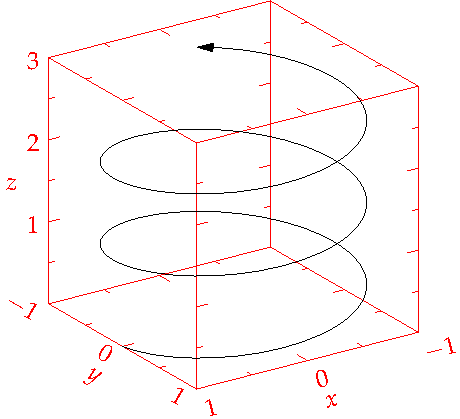
\includegraphics[width=\linewidth]{helix}
  \caption{This is a margin figure.  The helix is defined by 
    $x = \cos(2\pi z)$, $y = \sin(2\pi z)$, and $z = [0, 2.7]$.  The figure was
    drawn using Asymptote (\url{http://asymptote.sf.net/}).}
  \label{fig:marginfig}
\end{marginfigure}

\begin{docspec}
\textbackslash begin\{marginfigure\}\\
  \qquad\textbackslash includegraphics\{helix\}\\
  \qquad\textbackslash caption\{This is a margin figure.\}\\
  \qquad\textbackslash label\{fig:marginfig\}\\
\textbackslash end\{marginfigure\}\\
\end{docspec}

The \docenv{marginfigure} and \docenv{margintable} environments accept an optional parameter \docopt{offset} that adjusts the vertical position of the figure or table.  See the ``\nameref{sec:sidenotes}'' section above for examples.  The specifications are:
\begin{docspec}
  \textbackslash{begin\{marginfigure\}[\docopt{offset}]}\\
  \qquad\ldots\\
  \textbackslash{end\{marginfigure\}}\\
  \mbox{}\\
  \textbackslash{begin\{margintable\}[\docopt{offset}]}\\
  \qquad\ldots\\
  \textbackslash{end\{margintable\}}\\
\end{docspec}

Figure~\ref{fig:fullfig} is an example of the \docenv{figure*}
environment and figure~\ref{fig:textfig} is an example of the normal
\docenv{figure} environment.

\begin{figure*}[h]
  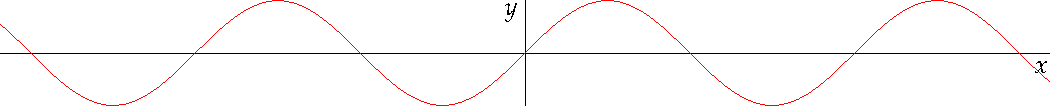
\includegraphics[width=\linewidth]{sine.pdf}%
  \caption{This graph shows $y = \sin x$ from about $x = [-10, 10]$.
  \emph{Notice that this figure takes up the full page width.}}%
  \label{fig:fullfig}%
\end{figure*}

\begin{figure}
  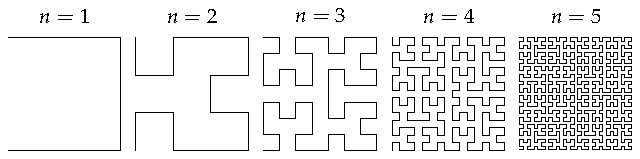
\includegraphics{hilbertcurves.pdf}
%  \checkparity This is an \pageparity\ page.%
  \caption[Hilbert curves of various degrees $n$.][6pt]{Hilbert curves of various degrees $n$. \emph{Notice that this figure only takes up the main textblock width.}}
  \label{fig:textfig}
  %\zsavepos{pos:textfig}
\end{figure}

\chapter{Conclusion}


%%
% The back matter contains appendices, bibliographies, indices, glossaries, etc.







\backmatter

\bibliography{biblio}
\bibliographystyle{plainnat}


\printindex

\end{document}

